\chapter{Probabilistic Circuits}
\label{chap:boolean_prob_circuits}

\section{Boolean Functions}
\label{sec:boolean_functions}

Let \(\mathbf{x} = (x_1, x_2, \dots, x_n)\) be a vector of \(n\) Boolean variables, where each \(x_i \in \{0,1\}\). A \emph{Boolean function} is a map
\begin{equation}
\label{eq:boolean_function}
F(\mathbf{x}) \;=\; F(x_1, x_2, \dots, x_n) \;\in\; \{0,1\}.
\end{equation}
This function takes each possible configuration of \(\mathbf{x}\) (i.e., each element of \(\{0,1\}^n\)) to a single binary output in~\(\{0,1\}\). Boolean functions appear throughout digital logic, circuit design, and a wide range of computational applications.

For illustration, we can visualize small Boolean functions based on the size of \(\mathbf{x}\). For \(n=1\), there are two possible input states:

\begin{center}
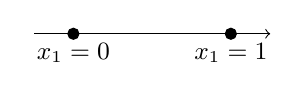
\begin{tikzpicture}
\filldraw[black] (0,0) circle (2pt) node[anchor=north]{\small $x_1=0$};
\filldraw[black] (2,0) circle (2pt) node[anchor=north]{\small $x_1=1$};
\draw[->] (-0.5,0) -- (2.5,0);
\end{tikzpicture}
\end{center}

For \(n=2\), the four possible states can be positioned on a 2D lattice:

\begin{center}
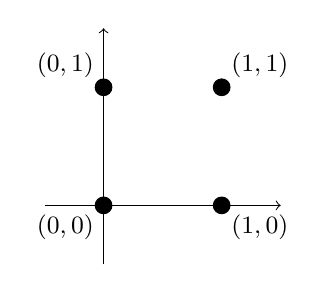
\begin{tikzpicture}[scale=1.5]
\filldraw[black] (0,0) circle (2pt) node[anchor=north east]{\small $(0,0)$};
\filldraw[black] (1,0) circle (2pt) node[anchor=north west]{\small $(1,0)$};
\filldraw[black] (0,1) circle (2pt) node[anchor=south east]{\small $(0,1)$};
\filldraw[black] (1,1) circle (2pt) node[anchor=south west]{\small $(1,1)$};
\draw[->] (-0.5,0) -- (1.5,0);
\draw[->] (0,-0.5) -- (0,1.5);
\end{tikzpicture}
\end{center}

In three dimensions (\(n=3\)), the eight possible states correspond to the vertices of a cube:

\begin{center}
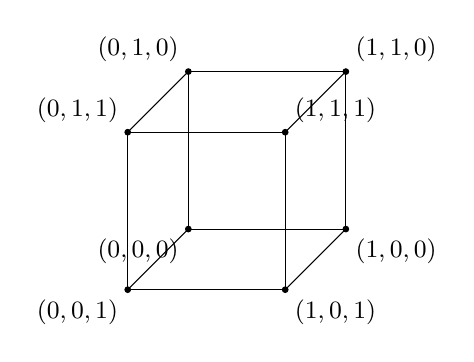
\begin{tikzpicture}[scale=2]
\coordinate (000) at (0,0,0);
\coordinate (001) at (0,0,1);
\coordinate (010) at (0,1,0);
\coordinate (011) at (0,1,1);
\coordinate (100) at (1,0,0);
\coordinate (101) at (1,0,1);
\coordinate (110) at (1,1,0);
\coordinate (111) at (1,1,1);

\foreach \point in {(000),(001),(010),(011),(100),(101),(110),(111)}
    \filldraw[black] \point circle (0.5pt);

\draw (000) -- (100) -- (110) -- (010) -- (000);
\draw (001) -- (101) -- (111) -- (011) -- (001);
\draw (000) -- (001);
\draw (100) -- (101);
\draw (110) -- (111);
\draw (010) -- (011);

\node[anchor=north east] at (000) {\small $(0,0,0)$};
\node[anchor=north west] at (100) {\small $(1,0,0)$};
\node[anchor=south east] at (010) {\small $(0,1,0)$};
\node[anchor=south west] at (110) {\small $(1,1,0)$};
\node[anchor=north east] at (001) {\small $(0,0,1)$};
\node[anchor=north west] at (101) {\small $(1,0,1)$};
\node[anchor=south east] at (011) {\small $(0,1,1)$};
\node[anchor=south west] at (111) {\small $(1,1,1)$};
\end{tikzpicture}
\end{center}

Boolean operators such as AND (\(\land\)), OR (\(\lor\)), and NOT (\(\lnot\)) allow constructing a wide variety of logical relationships. For example, in a setting where a system fails if any one of two components fails, the Boolean function can be written as
\[
F(x_A, x_B) \;=\; x_A \;\lor\; x_B.
\]
Here, \(F=1\) precisely when \(x_A=1\) or \(x_B=1\), encompassing a failure event if either component \(A\) or \(B\) is in state 1. More complex systems with many interdependent components may require Boolean functions with numerous variables and deeply nested operators.

Although Boolean functions are crucial for representing logical configurations, they operate purely in a binary framework and do not directly encode probability distributions. To include probabilistic behavior, we can move to a more expressive framework called \emph{probabilistic circuits}, which describe the distribution of variables in a directed acyclic graph (DAG). Such representations can capture both the combinatorial structure of system states and the uncertainty or likelihood associated with these states.

\section{Definition and Structure}

Consider a set of random variables \(\mathbf{X} = (X_1, X_2, \dots, X_n)\). A \emph{probabilistic circuit} \(\mathcal{C}\) is a DAG whose nodes consist of:

\begin{itemize}
 \item \textbf{Input nodes (leaves):} Each leaf encodes a base distribution over some subset of \(\mathbf{X}\). Often, these leaves correspond to univariate distributions \(p(X_i)\) or constant/indicator functions.
 \item \textbf{Internal nodes (gates):} Each gate combines incoming distributions from its children using either:
   \begin{itemize}
   \item \textbf{Sum-gates (mixture gates):} Weighted sums of child distributions, with nonnegative weights summing to 1.
   \item \textbf{Product-gates:} Factorized products of child distributions, each child covering disjoint subsets of \(\mathbf{X}\).
   \end{itemize}
\end{itemize}
The acyclic nature of the graph ensures that information flows consistently from the leaves toward a designated \emph{root} node.

\subsection{Sum-Gates and Product-Gates}

Let \(v\) be an internal node in \(\mathcal{C}\). Denote the children of \(v\) by \(\operatorname{ch}(v)\). Then:

\begin{itemize}
\item \textbf{Sum-gate:} Suppose \(v\) has children \(u_1,\dots,u_k\) with mixture weights \(\{\theta_{v,u_i}\}_{i=1}^k\) satisfying \(\sum_{i=1}^k \theta_{v,u_i} = 1\) and \(\theta_{v,u_i} \ge 0\). The distribution encoded at \(v\) is
\begin{equation}
\label{eq:sum_gate}
p_v(\mathbf{x}) \;=\; \sum_{i=1}^k \theta_{v,u_i}\,p_{u_i}(\mathbf{x}),
\end{equation}
where \(p_{u_i}(\mathbf{x})\) is the distribution encoded by child node \(u_i\).

\item \textbf{Product-gate:} Suppose \(v\) has children \(u_1,\dots,u_k\), each covering disjoint subsets of \(\mathbf{X}\). Let \(\mathbf{X}=\bigcup_{i=1}^k \mathbf{X}_{u_i}\) and \(\mathbf{X}_{u_i}\cap \mathbf{X}_{u_j} = \varnothing\) for \(i\neq j\). Then the distribution at \(v\) is
\begin{equation}
\label{eq:product_gate}
p_v(\mathbf{x})
\;=\;
\prod_{i=1}^k
p_{u_i}\bigl(\mathbf{x}_{u_i}\bigr),
\end{equation}
where \(\mathbf{x}_{u_i}\) is the restriction of \(\mathbf{x}\) to the variables in \(\mathbf{X}_{u_i}\).
\end{itemize}

\subsection{Leaf Nodes and the Circuit Distribution}

Each leaf node encodes a base distribution over its subset of variables (or a constant/indicator). Let \(v\) be a leaf node associated with \(p_v(\mathbf{X}_v)\). When the circuit is evaluated, each leaf contributes its assigned distribution or constant term. By recursively composing sum-gates and product-gates, every node \(v\) in the circuit defines a distribution \(p_v(\mathbf{x})\). The distribution of the entire circuit is given by evaluating its \emph{root} node \(r\):
\[
p_r(\mathbf{x}) \;=\; \text{(\(r\) evaluated from the leaves up)}.
\]

Probabilistic circuits unify structural and probabilistic modeling in a single formalism. They are widely used in fields such as artificial intelligence, machine learning, and automated reasoning, offering a tractable way to represent complex, high-dimensional probability distributions while preserving interpretable, compositional structure.